
\begin{figure*}
\begin{center}
%\hspace*{-1.3cm}
%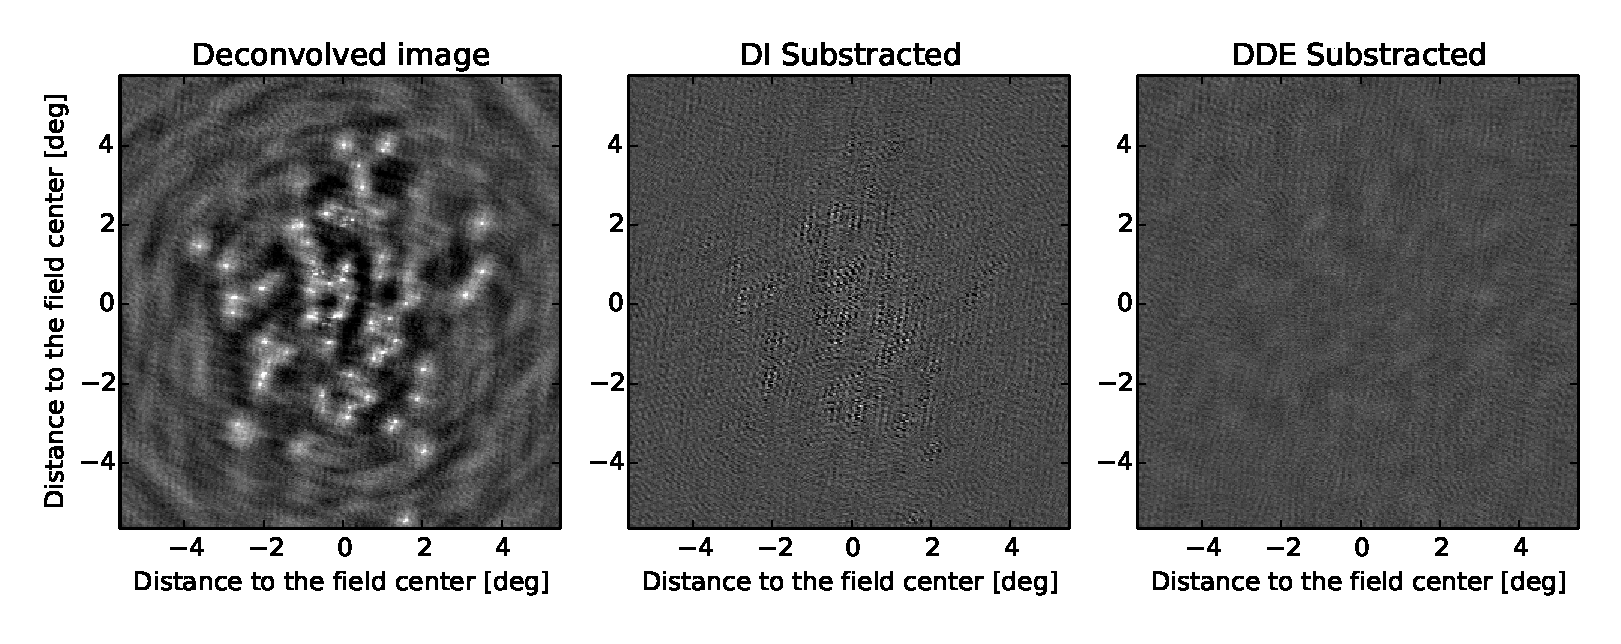
\includegraphics[width=\textwidth]{residSim.eps}
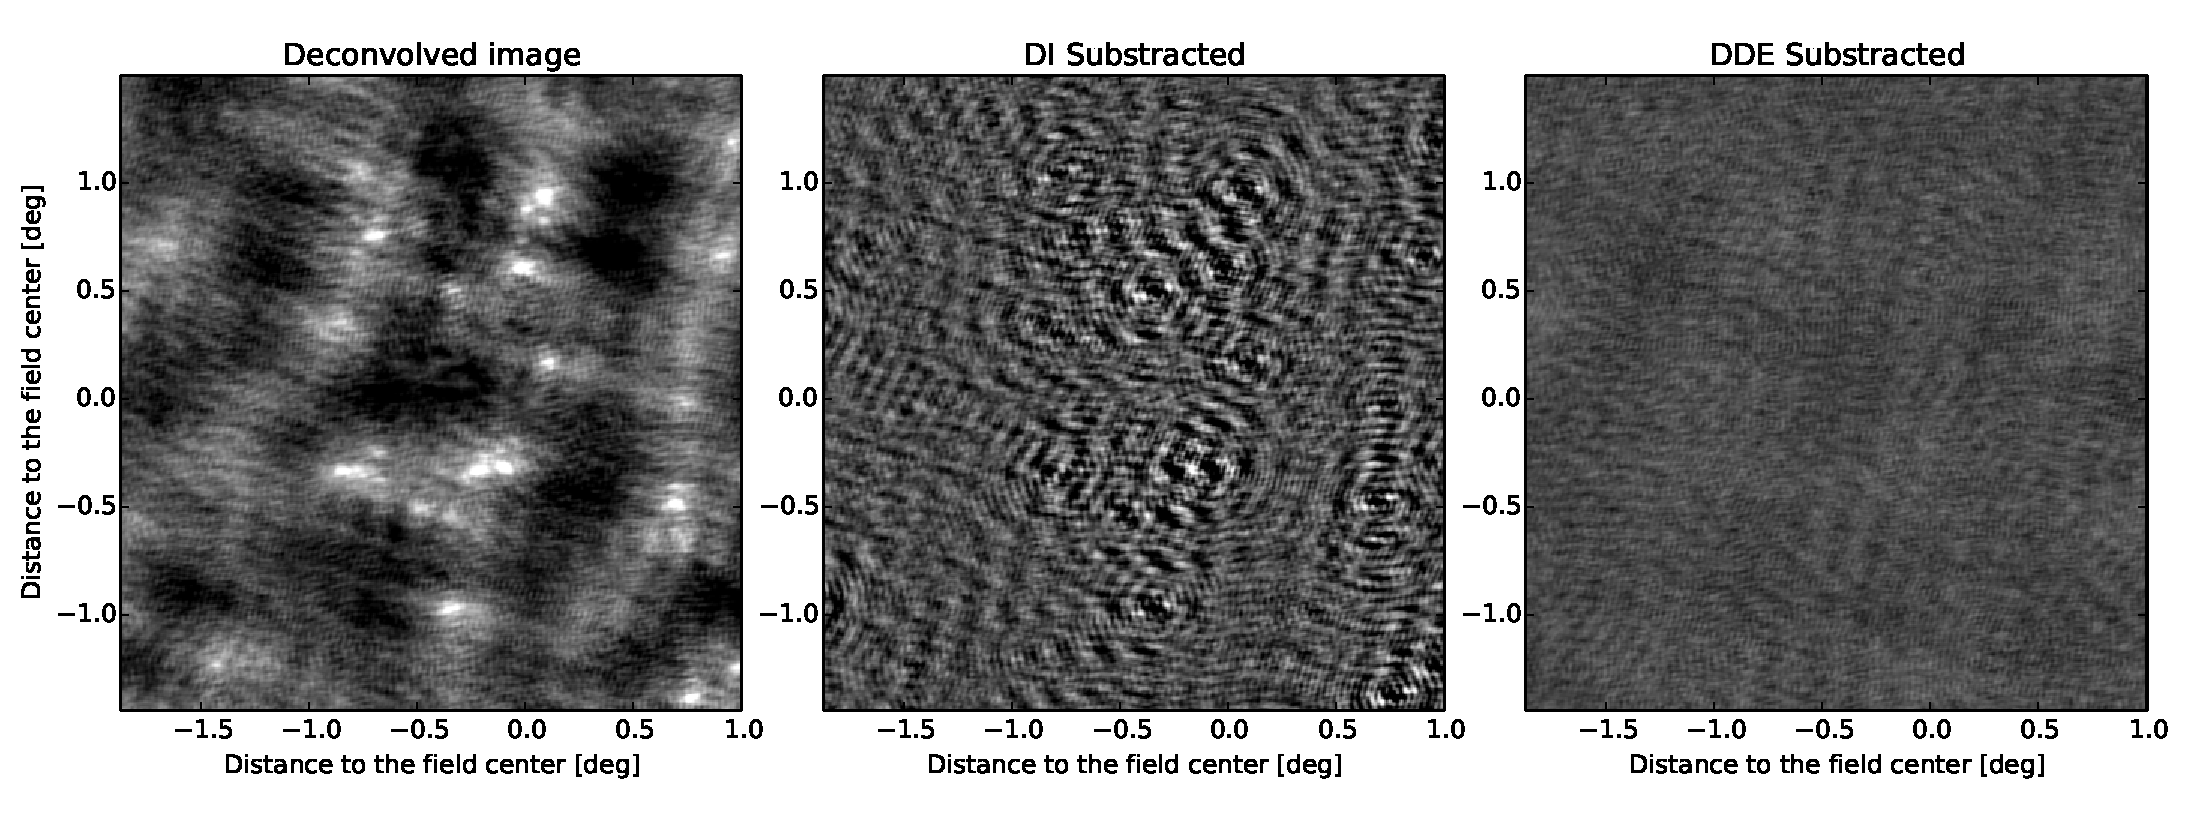
\includegraphics[width=\textwidth]{residSimZoom2.eps}
\caption{\label{fig:resid} This figure shows compares the image
  (left), the residuals data after simple skymodel substraction
  (center), and the residuals data after substracting the
  sky model corrupted by the direction-dependent solution (right).}
\end{center}
\end{figure*}


\section{Testing \COH on simulated data}

\subsection{Constant gains}
\label{sec:SimpleSimul}

A visibility dataset is simulated assuming the Low Frequency Array (LOFAR) antenna
layout. The phase center is located at
$(\alpha,\delta)=(14^h11^m20.5^s, +52^{o}12\arcmin10.0\arcsec)$,
observting frequency is $50$ MHz time
bins are 10 sec wide, and using a sky model containing five
sources, distributed in a cross. The gains applied to the antenna $p$ are
constant through time, and are taken at random along a normal distribution
$g_{p}\sim\mathcal{N}\left(0,1\right)+i\mathcal{N}\left(0,1\right)$.

The matrix corresponding matrix $\JVg^H\JVg$ is shown in
Fig. \ref{fig:HalfJHJ}. The calibration solution convergence are shown
in Fig. \ref{fig:Convergence}.



\subsection{Variable gains}
\label{sec:VarSimul}

In order to simulate a more realistic dataset, we use a 100 sources
skymodel. The gains are simulated assuiming an ionospheric
model consisting
of a purely scalar, direction-dependent phase (an infinitesimally thin layer at a height of 100 km). The
total electron content (TEC) values at a set of sample points are
generated using Karhunen-Loeve decomposition \citep[the spatial correlation
is given by Kolmogorov turbulence, see][]{Tol09}. The sources are clustered in 10 directions using Voronoi
tesselation.

Fig. \ref{fig:resid} shows the residuals the residuals as
computed by substracting the model data in the visibility domain, and
the model data affected by DDEs. Clearly, \textsc{cohjones} gives a
significant improvement over direct substraction.




%% \begin{figure*}
%% \begin{center}
%% %\hspace*{-1.3cm}
%% 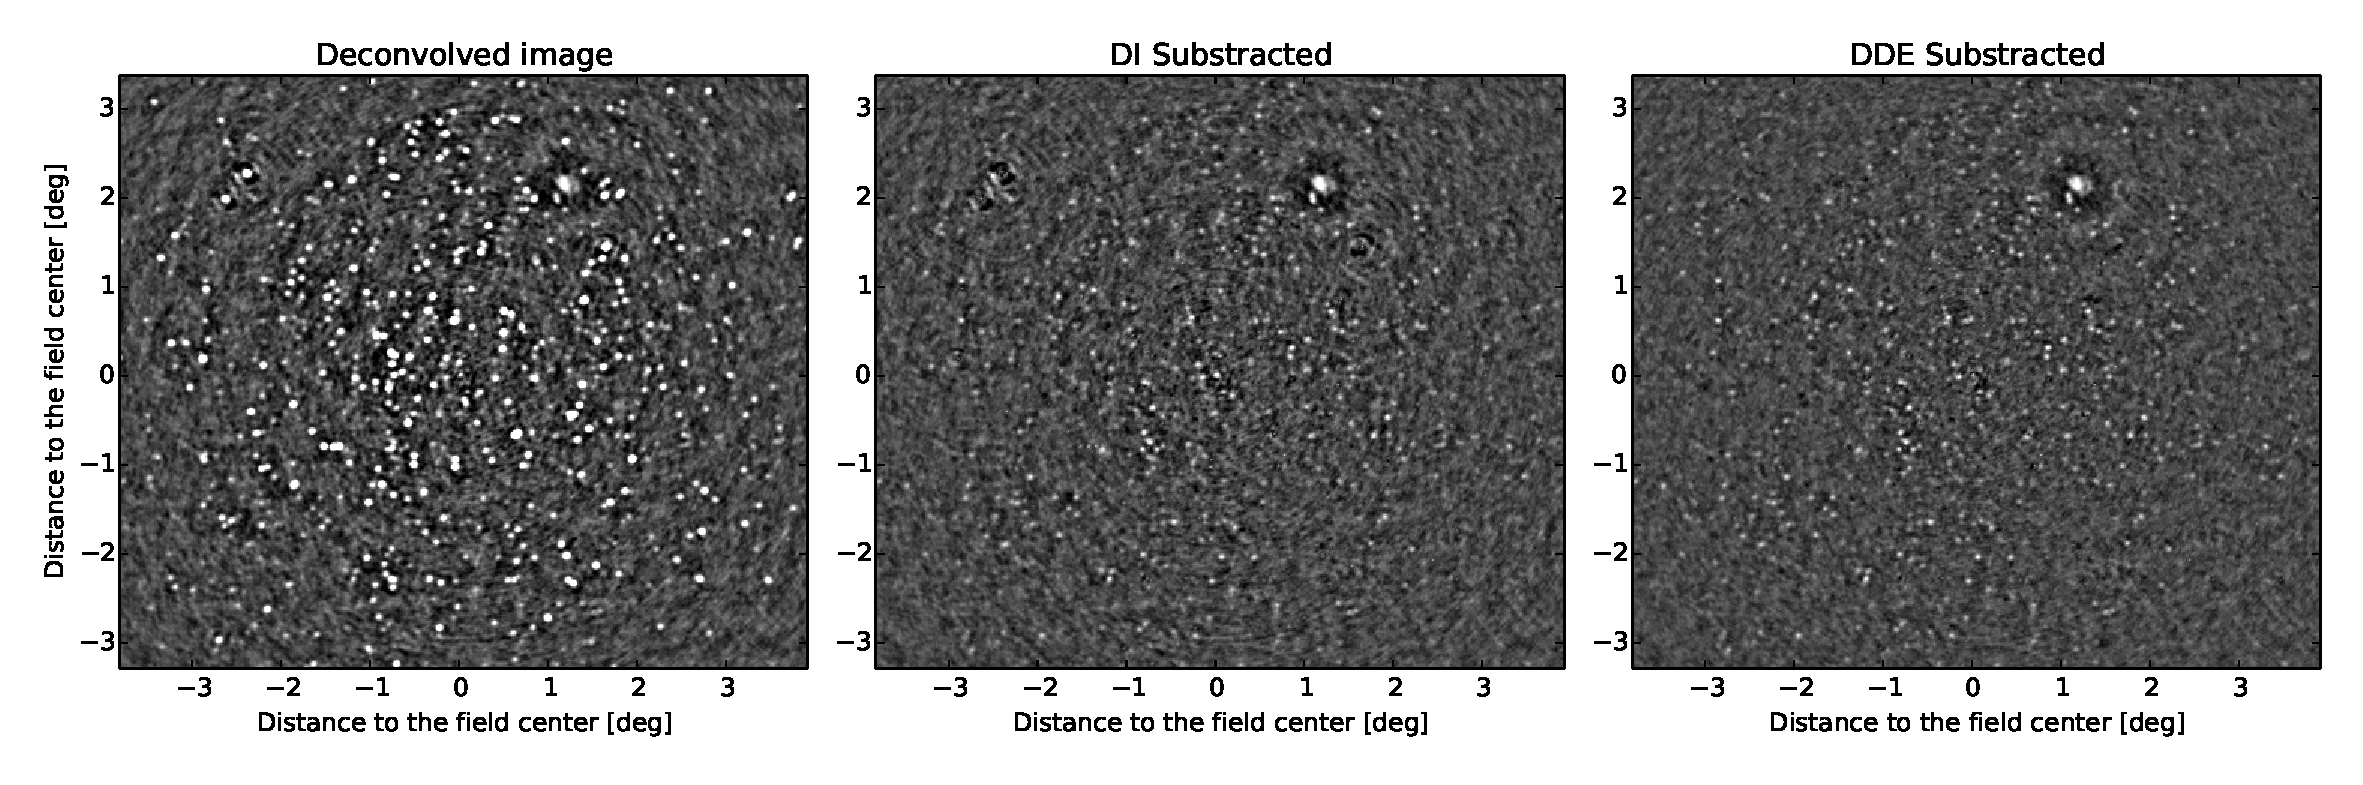
\includegraphics[width=\textwidth]{resid}
%% 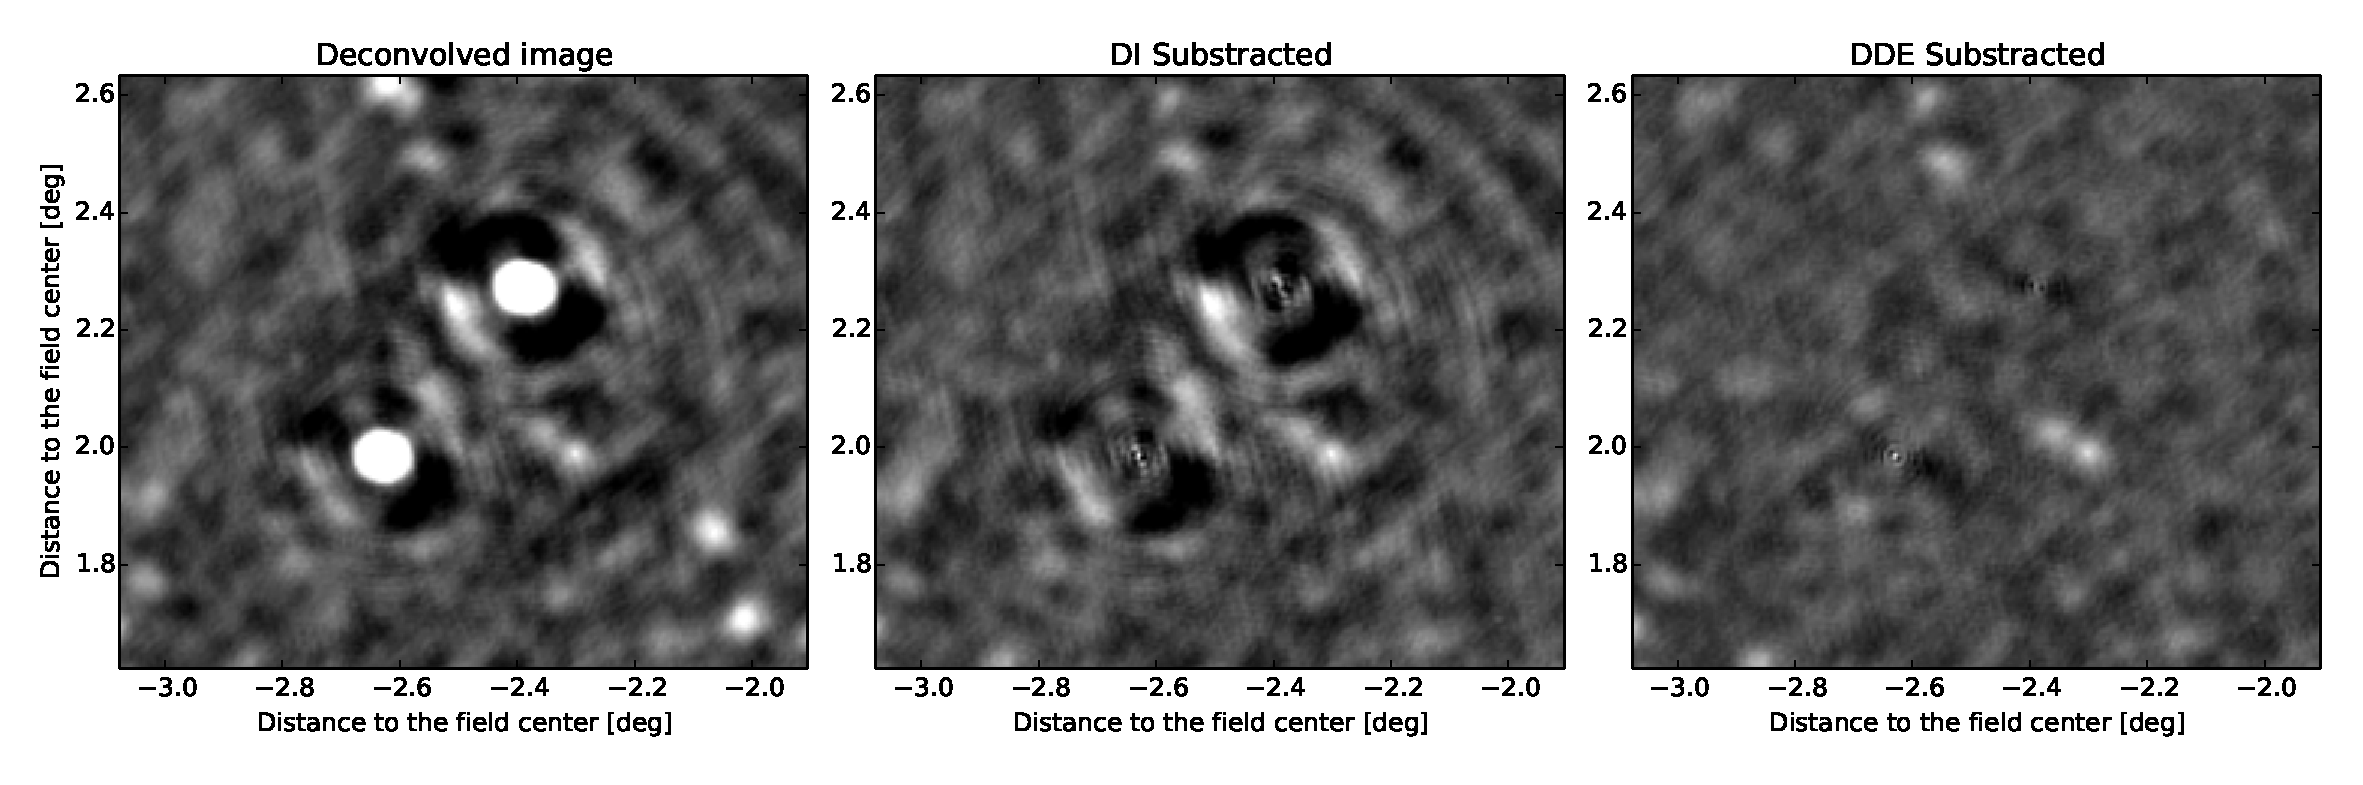
\includegraphics[width=\textwidth]{residZoom}
%% \caption{\label{fig:resid} This figure shows compares the image
%%   (left), the residuals data after simple skymodel substraction
%%   (center), and the residuals data after substracting the
%%   sky model corrupted by the direction-dependent solution (right).}
%% \end{center}
%% \end{figure*}

